\documentclass[12pt,letterpaper]{exam}
\usepackage[lmargin=1in,rmargin=1in,tmargin=1in,bmargin=1in]{geometry}
\usepackage{../style/exams}

% -------------------
% Course & Exam Information
% -------------------
\newcommand{\course}{MATH 141: Final Exam}
\newcommand{\term}{Fall --- 2025}
\newcommand{\examdate}{12/08/2025}
\newcommand{\timelimit}{150 Minutes}

\setbool{hideans}{false} % Student: True; Instructor: False

\usepackage{cancel}
\newcommand{\fixedunderline}[2]{%
\leavevmode
\makebox[#1][c]{%
   \begin{minipage}[t]{#1}\centering
	\strut #2\\[-1.7ex] % Adjust to move relative to text
	\rule{\linewidth}{0.4pt} % Adjust Thickness
   \end{minipage}%
  }%
}


% -------------------
% Content
% -------------------
\begin{document}

\examtitle
\instructions{Write your name on the appropriate line on the exam cover sheet. This exam contains \numpages\ pages (including this cover page) and \numquestions\ questions. Check that you have every page of the exam. Answer the questions in the spaces provided. Be sure to follow instructions, answer every question completely, and show all your work.} 
\scores
\bottomline
\newpage

% Poem
\phantom{.} \vfill
	\begin{table}[h]
	\centering
	\begin{tabular}{l}
	{\itshape ’Twas the night before Christmas, all frozen and still,} \\
	{\itshape Santa is working hard, but Math makes him quite ill.} \\
	{\itshape The sleigh is loaded, and the reindeer are prepared,} \\ 
	{\itshape But with problems unsolved, no gifts can be shared.} \\
	\\
	{\itshape ``These problems are hard!'', Santa cried out in fright.} \\
	{\itshape ``It's clear all my derivatives and sums aren't right!''} \\
	{\itshape This math needs to be done before Santa can take flight,} \\
	{\itshape He'll need a Calculus ace to help Save Christmas tonight!}
	\end{tabular}
	\end{table}
\phantom{.} \vfill 

% -------------------
% Questions
% -------------------
\begin{questions}

% Question 1
\newpage
\question[8] {\itshape On the brink of his flight, Santa is overcome with dismay, \par\phantom{(XX point)} For he'd forgotten his derivatives, quick, he needs help right away!} \par\vspace{0.3cm}
Find each of the following: \par\vspace{0.3cm}
	\begin{enumerate}[(a)]
	\item $\dfrac{d}{dx}\, \big( \cot x \big)= \vsol{-\csc^2 x}$ \vfill
	\item $\dfrac{d}{dx}\, \big( \ln x \big)= \vsol{\dfrac{1}{x}}$ \vfill
	\item $\dfrac{d}{dx}\, \big( \sec^{-1} x \big)= \vsol{\dfrac{1}{|x| \sqrt{x^2 - 1}}}$ \vfill
	\item $\dfrac{d}{dx}\, \big( \sec x \big)= \vsol{\sec x \tan x}$ \vfill
	\item $\dfrac{d}{dx}\, \big( \sin^{-1} x \big)= \vsol{\dfrac{1}{\sqrt{1 - x^2}}}$ \vfill
	\item $\dfrac{d}{dx}\, \big( \tan x \big)= \vsol{\sec^2 x}$ \vfill
	\item $\dfrac{d}{dx}\, \big( \tan^{-1} x \big)= \vsol{\dfrac{1}{1 + x^2}}$ \vfill
	\item $\dfrac{d}{dx}\, \big( \csc x \big)= \vsol{-\csc x \cot x}$
	\end{enumerate}



% Question 2
\newpage
\question[8] {\itshape Asked if he knew his derivatives, Santa sat in silence, thinking it through. \par\phantom{(XX point)} He shouted ``67!''. The elves let out a groan, “Okay, so we're not passing you.''} \par\vspace{0.3cm}
 
Showing all your work, compute the following derivatives---{\itshape do not simplify your answer}: \par\vspace{0.75cm}
	\begin{enumerate}[(a)]
	\item $\dfrac{d}{dx} \,\big( \sqrt{x^5} \arctan(2x) \big) \vsol{\;= \dfrac{d}{dx} \left( x^{5/2} \arctan(2x) \right)= \boxed{\frac{5}{2}\, x^{3/2} \cdot \arctan(2x) + \left( \dfrac{1}{1 + (2x)^2} \cdot 2 \right) \cdot x^{5/2}}}$ \vfill
	\item $\dfrac{d}{dx} \, \left( \dfrac{\tan(8x)}{\ln x} \right) \vsol{\;= \boxed{\dfrac{\big( \sec^2(8x) \cdot 8 \big) \cdot \left( \ln x \right) - \left( \dfrac{1}{x} \right) \cdot \left( \tan(8x) \right)}{(\ln x)^2}}}$ \vfill
	\item $\dfrac{d}{dx} \, \big( \, \sec^2(x^3) \,\big) \vsol{\;= \boxed{2 \sec(x^3) \cdot \big( \sec(x^3) \tan(x^3) \big) \cdot 3x^2}}$ \vfill
	\end{enumerate}



% Question 3
\newpage
\question[8] {\itshape Though Rudolph's red nose shone brightly, it dims at the limits ahead, \par\phantom{(XX point)} Santa needs help! Quick, compute these limits or Christmas could be dead!} \par\vspace{0.3cm}

Showing all your work, compute the limits below. {\bfseries You may not use l'H\^opital's rule.} \par\vspace{0.25cm}
	\begin{enumerate}[(a)]
	\item $\ds\lim_{x \to 9^-} \dfrac{x - 5}{x - 9} \psol{\;= \lim_{x \to 9^-} \dfrac{\overbrace{\strut x - 5}^{+}}{\underbrace{\strut x - 9}_{-}}= \boxed{-\infty}}$ \vfill
	\item $\ds\lim_{x \to 2} \dfrac{\;\; \frac{1}{x} - \frac{1}{2} \;\;}{x - 2} \vsol{\;= \lim_{x \to 2} \dfrac{\;\;\frac{2}{2x} - \frac{x}{2x}\;\;}{x - 2}= \lim_{x \to 2} \dfrac{\;\;\frac{2 - x}{2x}\;\;}{x - 2}= \lim_{x \to 2} \dfrac{\cancel{2 - x}^{\;\phantom{}^{\;\;-1}}}{2x \cancel{(x - 2)}}= \lim_{x \to 2} \dfrac{-1}{2x}= \dfrac{-1}{2(2)}= \boxed{-\dfrac{1}{4}}}$ \vfill
	
	\newpage\phantom{}\vspace{0.4cm}
	
	\item $\ds\lim_{x \to \infty} \dfrac{16x^3 + 1}{9 - 4x^3} \vsol{\;= \lim_{x \to \infty} \dfrac{16x^3 + 1}{9 - 4x^3} \cdot \dfrac{1/x^3}{1/x^3}= \lim_{x \to \infty} \dfrac{\;\;\frac{16x^3}{x^3} + \frac{1}{x^3}\;\;}{\frac{9}{x^3} - \frac{4x^3}{x^3}}= \lim_{x \to \infty} \dfrac{\;\;16 + \frac{1}{x^3}\;\;}{\frac{9}{x^3} - 4}= \dfrac{16 + 0}{0 - 4}= \boxed{-4}}$ \par\vspace{9.8cm}
	\item $\ds\lim_{x \to 9} \dfrac{x - 9}{3 - \sqrt{x}} \vsol{\;= \lim_{x \to 9} \dfrac{x - 9}{3 - \sqrt{x}} \cdot \dfrac{3 + \sqrt{x}}{3 + \sqrt{x}}= \lim_{x \to 9} \dfrac{\cancel{(x - 9)}^{\;\;\phantom{}^{-1}}(3 + \sqrt{x})}{\cancel{9 - x}}= \lim_{x \to 9} -(3 + \sqrt{x})= \boxed{-6}}$ \par\vspace{0.5cm}\begin{center} \vsol{{\itshape OR}} \end{center} \par\vspace{0.5cm} \vsol{\scalebox{1}{$\ds\lim_{x \to 9} \dfrac{x - 9}{3 - \sqrt{x}}= \lim_{x \to 9} \dfrac{(\sqrt{x} - 3)(\sqrt{x} + 3)}{3 - \sqrt{x}}= \lim_{x \to 9} \dfrac{\cancel{(\sqrt{x} - 3)}^{\;\;\phantom{}^{-1}}(\sqrt{x} + 3)}{\cancel{3 - \sqrt{x}}}= \lim_{x \to 9} -(\sqrt{x} + 3)= \boxed{-6}$}}
	\end{enumerate}



% Question 4
\newpage
\question[8] {\itshape Five golden rings, four calling birds, three French hens, \par\phantom{(XX point)} Two turtle doves, and a partridge in a pear tree! \par\phantom{(XX point)} \dots but they were all of them deceived for another ring was made.} \par
	\[
	\fbox{
	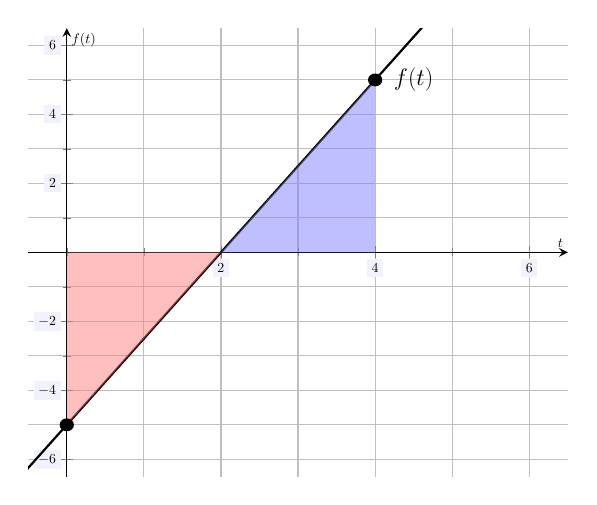
\begin{tikzpicture}[scale=1,every node/.style={scale=0.5}]
	\begin{axis}[
	grid=both,
	axis lines=middle,
	ticklabel style= {fill= blue!5!white},
	xmin= -0.5, xmax=6.5,
	ymin= -6.5, ymax=6.5,
	xtick= {-6,-4,...,6},
	ytick= {-8,-6,...,8},
	minor tick = {-10,-9,...,10},
	xlabel= \(t\), ylabel= \(f(t)\)
	]
	\node at (4.5,5) {\LARGE$f(t)$};
	\addplot[thick, samples=100, smooth, domain= -10.5:10.5] ({x},{5/2*x - 5});
	\vsol{\draw[draw=none,fill=red!50,opacity=0.5] (0,-5) -- (2,0) -- (0,0) -- (0,-5);}
	\vsol{\draw[draw=none,fill=blue!50,opacity=0.5] (2,0) -- (4,0) -- (4,5) -- (2,0);}
	\vsol{\draw[fill=black] (4,5) ellipse (0.085 and 0.17);}
	\vsol{\draw[fill=black] (0,-5) ellipse (0.085 and 0.17);}
	\end{axis}
	\end{tikzpicture}
	}
	\]
Let $\ds g(x)= \int_0^x f(t) \;dt$. Use the plot of $f(t)$ above to answer the following questions: \par\vspace{0.3cm}
	\begin{enumerate}[(a)]
	\item $g(2) \psol{\;\ds= \int_0^2 f(t) \;dt= -\frac{1}{2} \,(2) \,5= \boxed{-5}}$ \vfill
	\item $g(4) \vsol{\;\ds= \int_0^4 f(t) \;dt= \int_0^2 f(t) \;dt + \int_0^4 f(t) \;dt= -5 + \frac{1}{2} \,(2)\,5= -5 + 5= \boxed{0}}$ \vfill
	\item $g'(4) \vsol{\;\ds= \dfrac{d}{dx} \;g(x) \bigg|_{x=4}= \dfrac{d}{dx} \int_0^x f(t) \;dt \bigg|_{x=4}= f(x) \bigg|_{x=4}= f(4)= \boxed{5}}$ \vfill
	\item $g''(2) \vsol{\;\ds= \dfrac{d}{dx} \; g'(x) \bigg|_{x=2}= \dfrac{d}{dx} \; f(x) \bigg|_{x=2}= f'(x) \bigg|_{x=2}= f'(2)= \dfrac{5 - (-5)}{4 - 0}= \dfrac{10}{4}= \boxed{\dfrac{5}{2}}}$ \vfill
	\end{enumerate}



% Question 5
\newpage
\question[8] {\itshape All through the night, ole Santa worked hard---pressing on with cheer. \par\phantom{(XX point)} Suddenly, Santa froze and gasped. He'd forgotten his integrals this year!} \par\vspace{0.3cm}
Find each of the following: \par\vspace{0.3cm}
	\begin{enumerate}[(a)]
	\item $\ds\int \tan x \;dx= \vsol{\boxed{\ln|\sec x| + C}= -\ln|\cos x| + C}$ \vfill
	\item $\ds\int \csc^2 x \;dx= \vsol{-\cot x + C}$ \vfill
	\item $\ds\int \dfrac{1}{x} \;dx= \vsol{\ln|x| + C}$ \vfill
	\item $\ds\int \sec x \;dx= \vsol{\ln|\sec x + \tan x| + C}$ \vfill
	\item $\ds\int \dfrac{dx}{1 + x^2}= \vsol{\arctan x + C}$ \vfill
	\item $\ds\int \cot x \;dx= \vsol{\ln|\sin x| + C}$ \vfill
	\item $\ds\int \csc x \;dx= \vsol{\boxed{\ln|\csc x - \cot x| + C}= -\ln|\csc x + \cot x|}$ \vfill
	\item $\ds\int \sin x \;dx= \vsol{-\cos x + C}$
	\end{enumerate}



% Question 6
\newpage
\question[8] {\itshape What Santa knew about continuity wasn't quite true. \par\phantom{(XX point)} Turns out, he's gonna need some help making it through!} \par\vspace{0.3cm}

A function $f(x)$ is given below.
	\[
	f(x)=
	\begin{cases}
	x + 2, & x < 1 \\
	4 - x^2, & x \geq 1
	\end{cases}
	\] \par
	
\begin{enumerate}[(a)]
\item Write an equation that would express the fact that $f(x)$ is continuous at $x= 1$. \par\vspace{0.6cm}
	\psol{\itshape A function $f(x)$ is continuous at $x= a$ if the limit there is the function value. Therefore, if $f(x)$ is continuous at $x= 1$, we know\dots}\par\vspace{0.3cm} \psol{\hfill $\boxed{f(1)= \lim_{x \to 1} f(x)}$ \hfill \phantom{}} \par\vspace{0.6cm}

\item Determine whether $f(x)$ is actually continuous at $x= 1$. Explain why or why not in terms of the equation you wrote in (a). \par\vspace{0.6cm}

\vsol{\itshape If $f(x)$ is continuous at $x= 1$, then we know from (a) that $\ds f(1)= \lim_{x \to 1} f(x)$. We merely need to compute the left and right side of this equality (to compute the limit, we compute the left and right hand limit) to see if they are the same. We have\dots\par\vspace{0.1cm}
	\[
	\begin{aligned}
	f(1)&= 4 - 1^2= 4 - 1= 3 \\
	\\
	\lim_{x \to 1^-} f(x)&= \lim_{x \to 1^-} (x + 2)= 1 + 2= 3 \\
	\\
	\lim_{x \to 1^+} f(x)&= \lim_{x \to 1^+} (4 - x^2)= 4 - 1^2= 3
	\end{aligned}
	\] \par\vspace{0.1cm}
Because the left and right hand limits are equal, we know that $\ds\lim_{x \to 1} f(x)= 3$. But then $\ds f(1)= \lim_{x \to 1} f(x)$, so that $f(x)$ is continuous at $x= 1$.}
\end{enumerate}



% Question 7
\newpage
\question[8] {\itshape ``These limits!'' cried Santa. ``I can't manage them all.'' \par\phantom{(XX point)} ``Turns out, I'm no good with l'H\^opital!''} \par\vspace{0.3cm}

Showing all your work, {\itshape\bfseries use l'H\^opital's rule} (along with any necessary algebra or `tricks') to compute the following limits: \par\vspace{0.3cm}
	\begin{enumerate}[(a)]
	\item $\ds\lim_{x \to 0} \dfrac{6x}{\sin(7x)} \vsol{\;\stackrel{\text{L.H.}}{=} \lim_{x \to 0} \dfrac{6}{\cos(7x) \cdot 7}= \dfrac{6}{7\cos(0)}= \dfrac{6}{7(1)}= \boxed{\dfrac{6}{7}}}$ \par\vspace{3.8cm}
	\item $\ds\lim_{x \to \infty} \dfrac{\sqrt{x}}{\ln x} \vsol{\;\stackrel{\text{L.H.}}{=} \lim_{x \to \infty} \dfrac{\;\;\frac{1}{2 \sqrt{x}}\;\;}{\frac{1}{x}}= \lim_{x \to \infty} \dfrac{x}{2 \sqrt{x}}= \lim_{x \to \infty} \dfrac{\sqrt{x}}{2}= \boxed{\infty}}$ \par\vspace{3.8cm}
	\item $\ds\lim_{x \to 0} (1 - 2x)^{1/x}$ \par
		\vsol{%
		\[
		\begin{aligned}
		L:&= \lim_{x \to 0} (1 - 2x)^{1/x} \\[0.1cm]
		\ln(L)&= \lim_{x \to 0} \ln(1 - 2x)^{1/x} \\[0.1cm]
		\ln(L)&= \lim_{x \to 0} \frac{1}{x} \cdot \ln(1 - 2x) \\[0.1cm]
		\ln(L)&= \lim_{x \to 0} \dfrac{\ln(1 - 2x)}{x} \\[0.1cm]
		\ln(L)&\stackrel{\text{L.H.}}{=} \lim_{x \to 0} \dfrac{\;\;\frac{1}{1 - 2x} \cdot -2\;\;}{1} \\[0.1cm]
		\ln(L)&= \lim_{x \to 0} \dfrac{-2}{1 - 2x} \\[0.1cm]
		\ln(L)&= \tfrac{-2}{1} \\[0.1cm]
		\ln(L)&= -2 \\[0.1cm]
		L&= \boxed{e^{-2}}
		\end{aligned}
		\]
		}
	\end{enumerate}



% Question 8
\newpage
\question[8] {\itshape For the naughtiest students, Krampus brought integrals to fear, \par\phantom{(XX point)} ``Solve these quickly or you'll be stuck in Calculus next year!''} \par\vspace{0.3cm}

Showing all your work, compute the following: \par\vspace{0.3cm}
	\begin{enumerate}[(a)]
	\item $\ds\int \dfrac{x^{7/2} + x - 1}{x} \;dx$ \par\vspace{0.75cm}
	
		\[
		\psol{\int \dfrac{x^{7/2} + x - 1}{x} \;dx= \int \left( x^{5/2} + 1 - \dfrac{1}{x} \right) \;dx= \boxed{\frac{2}{7} \; x^{7/2} + x - \ln|x| + C}}
		\] \par\vspace{3.5cm}

	
	\item $\ds\int \sin^2 \theta \;d\theta$ \par\vspace{0.3cm}
		\vsol{%
		\itshape We know that $\sin^2 \theta= \frac{1 - \cos(2\theta)}{2}$. But then\dots
			\[
			\int \sin^2 \theta \;d\theta= \int \frac{1 - \cos(2\theta)}{2} \;d\theta= \dfrac{1}{2} \int 1 - \cos(2\theta) \;d\theta
			\]
		We know that $\ds\int 1 \;d\theta= \theta + C$. We now have to compute $\ds\int \cos(2\theta) \;d\theta$. Let $u= 2 \theta$, so that $du= 2 \;d\theta$. But then\dots
			\[
			\int \cos(2\theta) \;d\theta= \dfrac{1}{2} \int \cos(2\theta) \cdot 2 \;d\theta= \dfrac{1}{2} \int \cos(u) \;du= \dfrac{1}{2} \sin(u) + C= \dfrac{\sin(2\theta)}{2} + C
			\]
		Therefore, we have\dots
			\[
			\begin{aligned}
			\int \sin^2 \theta \;d\theta&= \dfrac{1}{2} \int 1 - \cos(2\theta) \;d\theta \\[0.2cm]
			&= \dfrac{1}{2} \left( \theta + \dfrac{\sin(2\theta)}{2} + C \right) \\[0.2cm]
			&= \boxed{\dfrac{\theta}{2} + \dfrac{\sin(2\theta)}{4} + C} \\[0.2cm]
			&= \dfrac{2\theta + \sin(2\theta)}{4} + C
			\end{aligned}
			\]
		}
	\end{enumerate}



% Question 9 
\newpage
\question[8] {\itshape Santa's Christmas looks ruined. This math is putting him in straits. \par\phantom{(XX. point)} All these diagrams confuse him, he needs helping reading off his rates!} \par\vspace{0.3cm}

Use the graph of the function below to answer the given questions.
	\[
	\fbox{
	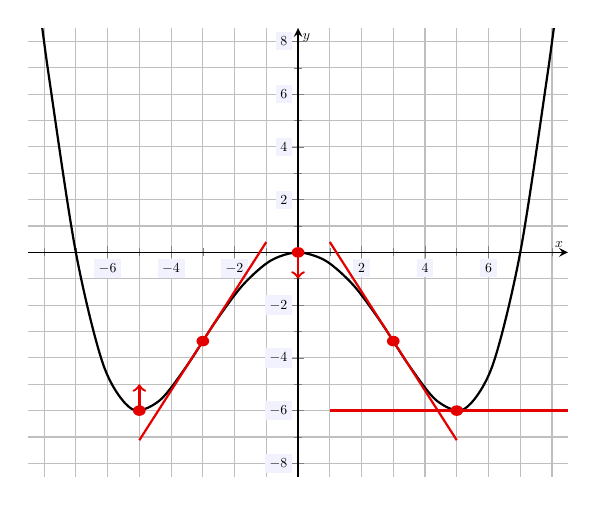
\begin{tikzpicture}[scale=1,every node/.style={scale=0.5}]
	\begin{axis}[
	grid=both,
	axis lines=middle,
	ticklabel style= {fill= blue!5!white},
	xmin= -8.5, xmax=8.5,
	ymin= -8.5, ymax=8.5,
	xtick= {-6,-4,...,6},
	ytick= {-8,-6,...,8},
	minor tick = {-10,-9,...,10},
	xlabel= \(x\), ylabel= \(y\)
	]
	\addplot[thick, smooth, domain= -10.5:10.5] ({x},{2*(-0.211547*x^2 + 0.00204939*x^4 + 0.0000834751*x^6 - 0.000000759007*x^8)});
	\vsol{\draw[draw=none,fill= red!90!black] (-5,-6) circle (0.2);}
	\vsol{\draw[line width=0.03cm,red!90!black,->] (-5,-6) -- (-5,-5);}
	\vsol{\draw[draw=none,fill= red!90!black] (-3,-3.3641) circle (0.2);}
	\vsol{\addplot[red!90!black, thick, smooth, domain= -5:-1] ({x},{-3.3641 + 1.879*(x + 3)});}
	\vsol{\draw[draw=none,fill= red!90!black] (0,0) circle (0.2);}
	\vsol{\draw[line width=0.03cm,red!90!black,->] (0,0) -- (0,-1);}
	\vsol{\draw[draw=none,fill= red!90!black] (3,-3.3641) circle (0.2);}
	\vsol{\addplot[red!90!black, thick, smooth, domain= 1:5] ({x},{-3.3641 - 1.879*(x - 3)});}
	\vsol{\draw[draw=none,fill= red!90!black] (5,-6) circle (0.2);}
	\vsol{\draw[line width=0.03cm,red!90!black,->] (1,-6) -- (9,-6);}
	\end{axis}
	\end{tikzpicture}
	}
	\]

\begin{enumerate}[(a)]
\item Assuming that a {\bfseries function $f(x)$} was plotted, indicate whether the following are positive ($ > 0$), negative ($< 0$), or equal to zero ($= 0$): \par\vspace{0.3cm}
	\begin{table}[!ht]
	\centering
	\begin{tabular}{rcr}
	$f''(-5)$ & \fixedunderline{2cm}{\vsol{$>$}} & $0$ \\[0.4cm]
	$f'(-3)$ & \fixedunderline{2cm}{\vsol{$>$}} & $0$ \\[0.4cm]
	$f''(0)$ & \fixedunderline{2cm}{\vsol{$<$}} & $0$ \\[0.4cm]
	$f'(3)$ & \fixedunderline{2cm}{\vsol{$<$}} & $0$ \\[0.4cm]
	$f'(5)$ & \fixedunderline{2cm}{\vsol{$=$}} & $0$ 
	\end{tabular}
	\end{table}

\item Assuming that a {\bfseries derivative $f'(x)$} was plotted, determine the following: \par\vspace{0.5cm}
	\hspace{0.3cm} Interval(s) where $f(x)$ is decreasing: \par\vfill
		\[
		\psol{\boxed{(-7, 0) \cup (0, 7)}}
		\] \par\vspace{0.3cm}\vfill
	
	\hspace{0.3cm} $x$-values of any local maxima/minima for $f(x)$: \par\vfill
		\[
		\psol{\boxed{x= -7\ \text{\itshape (local max)}, \; x= 7\ \text{\itshape (local min)}}\, , \; x= 0\ \text{\itshape (neither)}}
		\] \par\vspace{0.3cm}\vfill
	
	\hspace{0.3cm} Interval(s) where $f(x)$ is concave up: \par\vfill
		\[
		\psol{\boxed{(-5, 0) \cup (5, \infty)}}
		\] \par\vspace{0.3cm}\vfill
\end{enumerate}



% Question 10
\newpage
\question[8] {\itshape Though the elves did their best, their calculations gave Santa a fright, \par\phantom{(XX point)} He ho'd, ``Bring help---these derivatives might ground us tonight!''} \par\vspace{0.3cm}

Use the definition of the derivative to find $f'(x)$, where $f(x)= x^2 - 3x + 1$. You may check your answer using `shortcut rules', but you \textit{must} use the derivative definition for credit. You \textit{may not} use l'H\^opital's rule. Be sure to show all your work. \pspace

\vsol{\itshape We know that $f'(x)= 2x - 3$. We should obtain this same answer using the definition of the derivative. The definition of the derivative is\dots
	\[
	f'(x):= \lim_{h \to 0} \dfrac{f(x + h) - f(x)}{h}
	\] \par\vspace{0.2cm}
Using the fact that $f(x)= x^2 - 3x + 1$, we have\dots
	\[
	\begin{aligned}
	f(x + h)&= (x + h)^2 - 3(x + h) + 1 \\[0.2cm]
	&= (x^2 + 2hx + h^2) + (-3x - 3h) + 1 \\[0.2cm]
	&= x^2 + 2hx + h^2 - 3x - 3h + 1 \\
	\\
	f(x)&= x^2 - 3x + 1
	\end{aligned}
	\] \par\vspace{0.2cm}
Therefore, we have\dots
	\[
	\begin{aligned}
	f'(x)&= \lim_{h \to 0} \dfrac{f(x + h) - f(x)}{h} \\[0.2cm]
	&= \lim_{h \to 0} \dfrac{(x^2 + 2hx + h^2 - 3x - 3h + 1) - (x^2 - 3x + 1)}{h} \\[0.2cm]
	&= \lim_{h \to 0} \dfrac{x^2 + 2hx + h^2 - 3x - 3h + 1 - x^2 + 3x - 1}{h} \\[0.2cm]
	&= \lim_{h \to 0} \dfrac{\cancel{x^2} + 2hx + h^2 - \cancel{3x} - 3h + \cancel{1} - \cancel{x^2} + \cancel{3x} - \cancel{1}}{h} \\[0.2cm]
	&= \lim_{h \to 0} \dfrac{2hx + h^2 - 3h}{h} \\[0.2cm]
	&= \lim_{h \to 0} \dfrac{2\cancel{h}x + h^{\cancel{2}} - 3\cancel{h}}{\cancel{h}} \\[0.2cm]
	&= \lim_{h \to 0} (2x + h - 3) \\[0.2cm]
	&= \boxed{2x - 3}
	\end{aligned}
	\]
}



% Question 11
\newpage
\question[8] {\itshape He sped through the sky in his sleigh with such wobble and strain, \par\phantom{(XX point)} Santa laughed, ``At this rate, I’m as safe as a budget Boeing plane!''} \par\vspace{0.3cm}

Santa's sleigh velocity is given in the table below in increments of 2 seconds. \par
	\begin{table}[!ht]
	\centering
	\begin{tabular}{r||cccccc}
	Time (s) & $0$ & $2$ & $4$ & $6$ & $8$ & $10$ \\ \hline
	Velocity (mi/s) & $0$ & $0.5$ & $1$ & $2$ & $2.5$ & $5$
	\end{tabular}
	\end{table} \par
Estimate the distance Santa's sleigh has traveled over this 10~second period as accurately as possible by using the time at the start of each time interval. Based on the data and explaining your reasoning, would you predict your estimate to be an underestimate or overestimate of the distance traveled? \pspace

\vsol{\itshape We know that the change in distance is given by $\Delta x= \ds\int_0^{10} v(t) \;dt$. We know that we can approximate this integral with Riemann sums---left, right, or midpoint. We also know that the smaller the width of the rectangles used, i.e. the more rectangles used, the more accurate the approximation. We are told to use the most accurate approximation, so that we will use the `narrowest' rectangles, i.e. the ones on the intervals $[0, 2]$, $[2, 4]$, $[4, 6]$, $[6, 8]$, $[8, 10]$. Because we are told to use the time at the start of each interval, i.e. the value on the left of each interval, we are using a left hand Riemann sum. We can sketch out what we are computing.
	\[
	\fbox{
	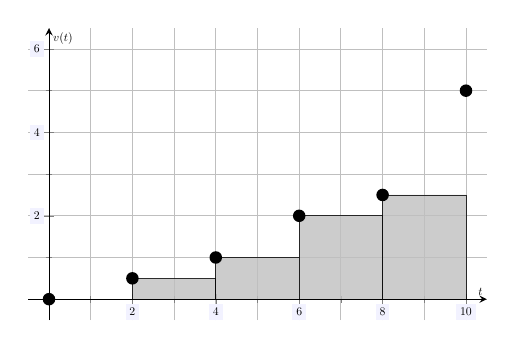
\begin{tikzpicture}[scale=0.85,every node/.style={scale=0.5}]
	\begin{axis}[
	axis equal image,
	grid=both,
	axis lines=middle,
	ticklabel style= {fill= blue!5!white},
	xmin= -0.5, xmax=10.5,
	ymin= -0.5, ymax=6.5,
	xtick= {-2,0,...,10},
	ytick= {-2,0,...,6},
	minor tick = {-10,-9,...,10},
	xlabel= \(t\), ylabel= \(v(t)\)
	]
	\draw[line width=0.3,fill=gray!50,opacity=0.8] (2,0) -- (2,0.5) -- (4,0.5) -- (4,0) -- (2,0);
	\draw[line width=0.3,fill=gray!50,opacity=0.8] (4,0) -- (4,1) -- (6,1) -- (6,0) -- (4,0);
	\draw[line width=0.3,fill=gray!50,opacity=0.8] (6,0) -- (6,2) -- (8,2) -- (8,0) -- (6,0);
	\draw[line width=0.3,fill=gray!50,opacity=0.8] (8,0) -- (8,2.5) -- (10,2.5) -- (10,0) -- (8,0);
	
	\draw[draw=none,fill=black] (0,0) circle (0.15);
	\draw[draw=none,fill=black] (2,0.5) circle (0.15);
	\draw[draw=none,fill=black] (4,1) circle (0.15);
	\draw[draw=none,fill=black] (6,2) circle (0.15);
	\draw[draw=none,fill=black] (8,2.5) circle (0.15);
	\draw[draw=none,fill=black] (10,5) circle (0.15);
	\end{axis}
	\end{tikzpicture}
	}
	\]
Therefore, we have\dots
	\[
	\Delta x= \ds\int_0^{10} v(t) \;dt \approx \sum f(x_i) \Delta x_i= 0(2) + 0.5(2) + 1(2) + 2(2) + 2.5(2)= 0 + 1 + 2 + 4 + 5= \boxed{12 \text{ mi}}
	\]
Each number added was of the form $\text{velocity} \cdot \text{time}$, which has units of $\text{mi/s} \cdot \text{s}$, so that the final answer has units of $\text{mi}$. Finally, because the velocity seems to be increasing, using the value at the start of each interval would likely be a smaller velocity than occurs over `most' of the interval. This would result in an underestimate of the distance traveled. Therefore, we have\dots
	\[
	\boxed{\text{Likely an underestimate because $v(t)$ appears to be increasing.}}
	\]

\vfill {\footnotesize Note. Traveling 12~mi in 10~seconds would be an average velocity of 1.2~mi/s. This is a speed of 4,320~mph---a hypersonic speed. This is twice as fast as the fastest manned operational jet---the SR-71 Blackbird. Santa's final speed of 5~mi/s is 18,000~mph---nearly the escape velocity for Earth!}}



% Question 12
\newpage
\question[8] {\itshape Santa hurtled through the sky, the fate of Christmas so near, \par\phantom{(XX point)} But he shook with fear, the integrals were too tricky to handle this year!} \par\vspace{0.3cm}

Showing all your work, compute the following integrals:
	\begin{enumerate}[(a)]
	\item $\ds\int_{-2}^1 x^2 \sqrt{x^3 + 8} \;dx$ \pspace
	
		\[
		\begin{aligned}
		\psol{u}&\psol{= x^3 + 8} &\hspace{2cm} \psol{x=1} &\psol{\colon} \quad \psol{u= 1^3 + 8= 9} \\[0.2cm]
		\psol{du}&\psol{= 3x^2 \;dx} & \psol{x= -2} &\psol{\colon} \quad \psol{u= (-2)^3 + 8= 0} \\
		\end{aligned}
		\] \par\vspace{0.5cm}
		
		\[
		\psol{\int_{-2}^1 x^2 \sqrt{x^3 + 8} \;dx= \dfrac{1}{3} \int_{-2}^1 \sqrt{x^3 + 8} \cdot 3x^2 \;dx= \dfrac{1}{3} \int_0^9 \sqrt{u} \;du}
		\]
	
		\[
		\psol{\hspace{3cm}=\dfrac{1}{3} \cdot \dfrac{2}{3}\; u^{3/2} \bigg|_0^9= \dfrac{2}{9}\; u^{3/2} \bigg|_0^9= \dfrac{2}{9} \left( 9^{3/2} - 0^{3/2} \right) = \dfrac{2}{9} \,(27 - 0)= 2(3)= \boxed{6}}
		\] \par\vspace{2.8cm}
	
	\item $\ds\int \dfrac{dx}{x \ln x}$ \pspace
	
		\[
		\begin{aligned}
		\psol{u}&\psol{= \ln x} \\[0.2cm]
		\psol{du}&\psol{= \dfrac{1}{x} \;dx} 
		\end{aligned}
		\] \par\vspace{0.5cm}
		
		\[
		\psol{\int \dfrac{dx}{x \ln x}= \int \dfrac{1}{\ln x} \cdot \dfrac{1}{x} \;dx= \int \dfrac{1}{u} \;du= \ln|u| + C= \boxed{\ln| \ln| x| \,| + C}}
		\]
	\end{enumerate}



% Question 13
\newpage
\question[8] {\itshape Santa's trajectory is not correct, ``Someone help me!'' \par\phantom{(XX point)} ``No one told me that I that couldn't use Chat-GPT!''} \par\vspace{0.3cm}

Find the equation of the tangent line to $x^3 + y^3= 9xy$ at the point $(2, 4)$. \pspace

\vsol{\itshape We know that the tangent line is given by $\ell(x)= y_0 + m(x - x_0)$. We know that $(x_0, y_0)= (2, 4)$. To find the slope, we have\dots
	\[
	\begin{gathered}
	x^3 + y^3= 9xy \\[0.2cm]
	\dfrac{d}{dx} \left( x^3 + y^3 \right)= \dfrac{d}{dx} \left( 9xy \right) \\[0.2cm]
	3x^2 + 3y^2 \cdot \dfrac{dy}{dx}= 9 \cdot y + 9x \cdot \dfrac{dy}{dx}
	\end{gathered}
	\]
Using the fact that we are at the point $(2, 4)$, we have\dots
	\[
	\begin{gathered}
	3x^2 + 3y^2 \cdot \dfrac{dy}{dx}= 9 \cdot y + 9x \cdot \dfrac{dy}{dx} \\[0.2cm]
	3(2^2) + 3(4^2) \cdot \dfrac{dy}{dx}= 9 \cdot 4 + 9(2) \cdot \dfrac{dy}{dx} \\[0.2cm]
	12 + 48\, \dfrac{dy}{dx}= 36 + 18\, \dfrac{dy}{dx} \\[0.2cm]
	30\, \dfrac{dy}{dx}= 24 \\[0.2cm]
	\dfrac{dy}{dx}= \dfrac{24}{30} \\[0.2cm]
	\dfrac{dy}{dx}= \dfrac{4}{5}
	\end{gathered}
	\]	
But then $m= \frac{4}{5}$. Therefore, the tangent line is\dots
	\[
	\ell(x)= y_0 + m(x - x_0)= \boxed{4 + \frac{4}{5}\,(x - 2)}= \dfrac{4x + 12}{5}
	\]
}



% Question 14
\newpage
\question[8] {\itshape They'd delivered presents and joy, against the winter cold moon bright. \par\phantom{(XX point)} Santa and his reindeer, no chance for relief, press on this Christmas night.} \par\vspace{0.3cm}

While Santa's sleigh rushes through the sky, a reindeer drops a Christmas `surprise.' It strikes a frozen pond, creating a circular hole in the ice that is 4~ft across. The hole freezes back over such that its radius decreases at a constant rate of 0.5~ft/min. After 2~minutes, at what rate is the area of this hole changing? Include units in your answer. \pspace

\vsol{\itshape
	\[
	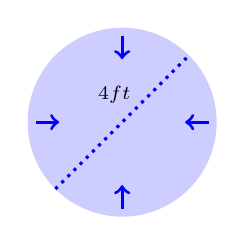
\begin{tikzpicture}
	\draw[draw=none,fill=blue!30,opacity=0.65] (0,0) circle (1.2);
	\draw[line width=0.04cm,blue,->] (0,-1.1) -- (0,-0.8);
	\draw[line width=0.04cm,blue,->] (1.1,0) -- (0.8,0);
	\draw[line width=0.04cm,blue,->] (0,1.1) -- (0,0.8);
	\draw[line width=0.04cm,blue,->] (-1.1,0) -- (-0.8,0);
	\draw[line width=0.04cm,blue,dotted] (-0.848528,-0.848528) -- (0.848528,0.848528);
	\node at (-0.1,0.35) {\scriptsize$4 \text{ ft}$};
	\end{tikzpicture}
	\]
We know that the hole is originally 4~ft across, i.e. a diameter of 4~ft. This means that the radius at the start is $r_0= \frac{4}{2}= 2$~ft. We know that the radius is decreasing at a rate of 0.5~ft/min, i.e. $\frac{dr}{dt}= -0.5$~ft/min. After 2~minutes, we know that the radius has changed by $\text{rate} \cdot \text{time}= -0.5 \cdot 2= -1$, so that the radius is $r= r_0 + \Delta r= 2 + (-1)= 1$~ft. This information is summarized below.
	\[
	\begin{aligned}
	d_0&= 4 \text{ ft} \\
	r_0&= \frac{d_0}{2}= \frac{4}{2}= 2 \text{ ft} \\
	\dfrac{dr}{dt}&= -0.5 \quad \text{\small *Constant} \\
	r&= r_0 + \Delta r= 2 + (-1)= 1 \text{ ft}
	\end{aligned}
	\]
We know that the area of the hole is given by $A= \pi r^2$. Therefore, we have\dots
	\[
	\begin{gathered}
	A= \pi r^2 \\
	\dfrac{d}{dt}\, A= \dfrac{d}{dt} \,(\pi r^2) \\
	\dfrac{dA}{dt}= 2\pi r \cdot \dfrac{dr}{dt} \\
	\dfrac{dA}{dt}= 2\pi (1 \text{ ft}) \cdot -0.5 \text{ ft/min} \\
	\dfrac{dA}{dt}= -\pi \text{ ft$^2$/min} \approx -3.14159 \text{ ft$^2$/min}
	\end{gathered}
	\]
Therefore, the area of the hole is decreasing at a rate of $\pi$ ft$^2$/min. 
	\[
	\boxed{-\pi \text{ ft$^2$/min} \approx -3.14 \text{ ft$^2$/min, i.e. decreasing at } \pi \text{ ft$^2$/min} \approx 3.14 \text{ ft$^2$/min}}
	\]
}



% Question 15
\newpage
\question[8] {\itshape With presents delivered and Christmas nearly in the clear, \par\phantom{(XX point)} Santa has one last task, and then you're done for this year!} \par\vspace{0.3cm}

With Christmas over, Santa needs to create a pen to house his reindeer until next year. The rectangular pen will be built alongside his toy factory. One side will be against the factory while the other three sides will be made of electrified steel fencing. He has 120~ft of fencing available. What is the area of the largest pen that Santa can build? Show all your work and be sure to prove that this area is indeed a maximum. \par\vspace{0.2cm}

\vsol{\small\itshape We first sketch the situation: \par
	\hfill\begin{minipage}{0.3\textwidth}
	\[
	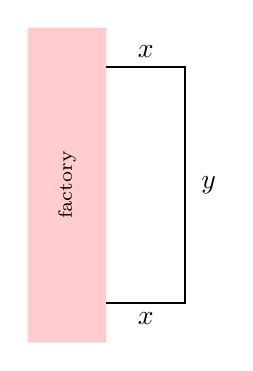
\begin{tikzpicture}
	\draw[draw=none,fill=red!30,opacity=0.65] (0,0) -- (1,0) -- (1,4) -- (0,4) -- (0,0);
	\node at (0.5,2) {\rotatebox{90}{\text{\scriptsize factory}}};
	\draw[line width=0.03cm] (1,3.5) -- (2,3.5) -- (2,0.5) -- (1,0.5);
	\node at (1.5,3.7) {$x$};
	\node at (1.5,0.3) {$x$};
	\node at (2.3,2) {$y$};
	\end{tikzpicture}
	\]
	\end{minipage}
	\begin{minipage}{0.3\textwidth}
		\[
		\begin{gathered}
		P= x + y + x \\
		P= 2x + y \\
		120= 2x + y \\
		y= 120 - 2x
		\end{gathered}
		\]
	\end{minipage} \hfill\phantom{} \par
To make the largest enclosure, we should use all the available fencing. We know the total fencing available is 120~ft, i.e. the perimeter of the fencing should be 120~ft. So, we know $P= 120 \text{ ft}$. We want to maximize the area of the enclosure, i.e. $A= \ell w= x y$. We can use the perimeter to solve for one variable in terms of the other, which we do above, to find the area in terms of one variable. We then have $A= xy= x(120 - 2x)= 120x - 2x^2$, i.e. the area is given in terms of $x$ by $A(x)= x(120 - 2x)= 120x - 2x^2$. Because there is only 120~ft of fencing available and the side $x$ consists of two sides the enclosure, we know that $x \in [0, \frac{120}{2}]= [0, 60]$. We find the maximum area by finding the critical values for $A(x)$. We know that $A'(x)= 120 - 2(2x)= 120 - 4x$. We know $A'(x)$ is never undefined. So, the only critical values will be where $A'(x)$ is $0$. But then\dots
	\[
	\begin{gathered}
	A'(x)= 0 \\
	120 - 4x= 0 \\
	4x= 120 \\
	x= 30 \text{ ft}
	\end{gathered}
	\]
Therefore, $y= 120 - 2x= 120 - 2(30)= 120 - 60= 60 \text{ ft}$. Now if $x= 0$, it must be that $y= 120$. If $x= 60$, then $y= 0$. We compare the area at our critical value to the area at the endpoints:
	\[
	A(0)= xy= 120(0)= 0 \text{ ft}^2, \quad A(30)= xy= 30(60)= 1,\!800 \text{ ft}^2, \quad A(60)= xy= 60(0)= 0 \text{ ft}^2
	\]
Therefore, the maximum area occurs when $x= 30 \text{ ft}$ and $y= 60 \text{ ft}$. We can confirm this is indeed a maximum by using the first derivative test:
	\[
	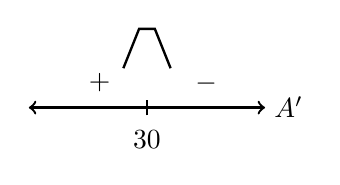
\begin{tikzpicture}
	\draw[line width=0.03cm,<->] (-1.5,0) -- (1.5,0); 
	\draw[line width=0.03cm] (0,-0.1) -- (0,0.1);
	\node at (0,-0.4) {$30$};
	\node at (1.8,0) {$A'$};
	\node at (-0.6,0.32) {$+$};
	\node at (0.75,0.3) {$-$};
	\draw[line width=0.03cm] (-0.3,0.5) -- (-0.1,1) -- (0.1,1) -- (0.3,0.5);
	\end{tikzpicture}
	\]
Using the second derivative test, we have $A''(x)= -4$, so that $A''(30)= -4 < 0$. In any case, we know the area of the largest possible enclosure is\dots
	\[
	\boxed{A= 1,\!800 \text{ ft}^2}
	\]
}
\end{questions}


% End Poem
\newpage

\phantom{.} \vfill
	\begin{table}[h]
	\centering
	\begin{tabular}{l}
	{\itshape The night was set right and magic of Christmas came true.} \\
	{\itshape Santa let out a sigh, these students really came through.} \\
	{\itshape Each limit untangled, each rate made precise,} \\
	{\itshape They restored all the magic that keeps Christmas nice.} \\
	\\
	{\itshape And Santa called out as he rode through the night,} \\
	{\itshape His voice full of cheer and his heart lifted light:} \\
	{\itshape ``Merry Christmas to all! But before I depart,} \\
	{\itshape Never forget your Calculus---the math of the heart!''} 
	\end{tabular}
	\end{table}
\phantom{.} \vfill

\end{document}